
\section{Deterministic Queueing Networks}
\label{sec:determ-queu-netw}

The simplest possible single-server queueing system is such that job
interarrival times are deterministic and that all service times are
equal. In such cases it is easy to determine the maximal throughput,
i.e., the capacity of the queueing system. Clearly, if the service
time is $t_1$, then the service rate is $r_1 = 1/t_1$. We can also
determine the minimal amount of jobs required to keep the server busy,
hence achieve maximal throughput.  We call this the \emph{critical
  work in progress (WIP)} and denote it by $W_0$. The minimal amount
of time needed to move from the start of the system to the end, also
called \emph{raw processing time} is denoted by $T_0$.  With Little's
law we can relate these two concepts for the single-server example.
If the arrival rate is equal to the service rate, then
$\lambda = r_1$, so that
\begin{equation*}
  W_0 = \lambda T_0 = r_1 T_0.
\end{equation*}
Since, in the single server case $T_0 = t_1$, we see that
$W_0=r_1 t_1 = t_1^{-1}t_1 = 1$. This result is evident: to get
maximal throughput, it is necessary that the server is always busy,
hence it must be that $W_0\geq 1$. Given that we deal with a $D/D/1$,
by assumption, we can tune the arrivals such that whenever a job
leaves, a new job arrives.

When we deal with \emph{networks}, determining $W_0$ and $T_0$ is not
so simple anymore. These quantities, however, are important to
know. It is not possible to organize the network such that jobs spend
less time than $T_0$ in the network. The raw processing time is the
sum of the required processing times and does not include, by
assumption, any queueing times. The critical WIP $W_0$ is important,
because if the network contains less jobs than this amount, throughput
will suffer. Stated in other terms, there not sufficient jobs in the
network to keep bottleneck machines fully loaded with work. For these
reasons $T_0$ and $W_0$ act as lower bounds on the time jobs spend in
the network and the amount of work required to achieve a certain
throughput.  Finally, it is important to know the bottleneck capacity
$r_b$ of the network: The maximal throughput of the network cannot
exceed the bottleneck capacity. Thus, when accepting jobs, one needs
to respect the capacity of the network. 

Before we study queueing networks in stochastic settings, we should
familiarize ourselves with the behavior of networks of queueing
systems in the simplest setting possible.  For this we need some
further definitions. A queueing network can be represented as
\emph{graph}. \emph{Stations} form the nodes in the graph, and edges
between nodes represents the possibility that jobs that can move from
one station to another. A simple example is a tandem network with two
stations. Jobs arrive at station~1 and after service they move to
station~2. After service at station~2, they leave the network. A
station can contain one or more servers. For instance, a single-server
station contains just one server. Finally, we assume that job service
times are constant at all servers at all stations. In other words,
service times need not be same from one machine/server or station
to another, but each server works at constant speed.  The
\emph{utilization} of station $i$ is the rate $\lambda_i t_i$, i.e.,
the rate at which work arrives, times the (average) service time per
job. The \emph{bottleneck} station is the station with the
\emph{highest utilization}.

As an example, consider $n$ single-server stations in tandem such that
the service time  at station $i$ is constant and equal to
$S$. Jobs arrive at rate $\lambda$. Then  the raw processing time 
\begin{equation*}
  T_0= n S.
\end{equation*}
Suppose now that we would release just one job in the system, in other
words, only when the first job has visited all stations, the next job
is released. In that case, the capacity $\mu$ of the network is
$1/T_0$. In general, a bit of thought will show that if we are
prepared to release $w$ jobs, then the capacity of the network is
given by
\begin{equation*}
  \mu(w) = \min\{w, n\} \frac 1{T_0}.
\end{equation*}
Thus, we need a minimal amount $w$ in the network to guarantee that
$\mu(w)> \lambda$. We also see that the maximal capacity of the
network is achieved when $w\geq n$, in which case,
\begin{equation*}
  \mu(w) = \frac{n}{T_0} = \frac{n}{n S} = \frac 1S.
\end{equation*}
Finally, for given $w$ we can maximize the waiting time by setting
$\lambda = \mu(w)$, and then by Little's law,
\begin{equation*}
  \begin{split}
  \E W 
= \frac{\E L}{\lambda} = \frac{w}{\mu(w)} = \frac{w}{\min\{w, n\}} T_0 
=
\begin{cases}
  T_0=nS, & \text{ if } w\leq n, \\
  \frac{w}{n} T_0 = w S, & \text{ if } w\geq n.
\end{cases}
  \end{split}
\end{equation*}
Thus, we see that $w>n$, there must be $w-n$ jobs in queue and the
other $n$ jobs are in service. So, in conclusion, in determinstic
tandem networks adding more than $n$ jobs does not increase the
network capacity, but only increases the waiting times. On the other
hand, setting $w<n$, minimizes the waiting times, but also negatively
affects the capacity.

The problems below are generalizations to networks with multi-server
stations, servers with different processing rates, and multiple
routings. They are meant to help you become acquainted with networking
behavior (and also Little's law, as we use this time and again
here). The problems appear much simpler than they are; I had much less
trouble making the problems than solving them. In fact, to ensure that
I got the answer right, I often tried to find two different ways to
solve the same problem. Be warned!

\begin{question}
  A production system consists of 2 separate stations. Jobs never go
  from one machine to another. The processing times are
  $(t_1, t_2) = (1, 2)$ hours. The arrival rates are
  $(\lambda_1, \lambda_2) = (1/3, 1/3)$ per hour. What is the fastest
  machine? Which machine is the bottleneck? 
  \begin{solution}
    The processing rates are $\mu_1=1/1$ and $\mu_2 = 1/2$ per hour,
    respectively. The utilizations $\rho_i=\lambda_i/\mu_i$ are $1/3$
    and $2/3$, respectively. Thus, machine 2 is the bottleneck: it has
    the highest utilization.

    Since these machines are not related by a routing (jobs going from
    one machine to another), computing $T_0$ and so on does not make
    much sense for the network. We can just consider each machine on
    its own. Then, as we need $2$ jobs to keep each machine busy, it
    follows that $W_0=2$. 

We can use Little's law to find $T_0$. The rate at which jobs can be served is $\mu = 1+1/2 = 3/2$. Thus, 
\begin{equation*}
  T_0 = W_0/\mu = 2/(3/2)=4/3.
\end{equation*}
Thus, the average time a job spends in this system is $4/3$ time units
if jobs arrive at the rate they are served. (Recall, everything is
deterministic.)

Can we see this in another way? Yes, because $2$ out of $3$ jobs have service time of $1$, and $1$ out of $3$ a service time of $2$. Thus,
\begin{equation*}
  \frac23 1 + \frac 1 3 2 = \frac 4 3.
\end{equation*}
  \end{solution}
\end{question}



\begin{question}
  A production network consists of 3 single-machine stations in
  tandem, i.e., in series, c.f. Figure~\ref{fig:tandemraw}. The
  processing times are $(2, 3, 2)$ hours respectively, i.e., constant
  and such that $t_1=2$ hours, $t_2=3$ hours and $t_3=2$ hours.

What are the critical WIP $W_0$, bottleneck
  capacity $r_b$ and raw processing time~$T_0$?

  \begin{figure}[ht]
    \centering
    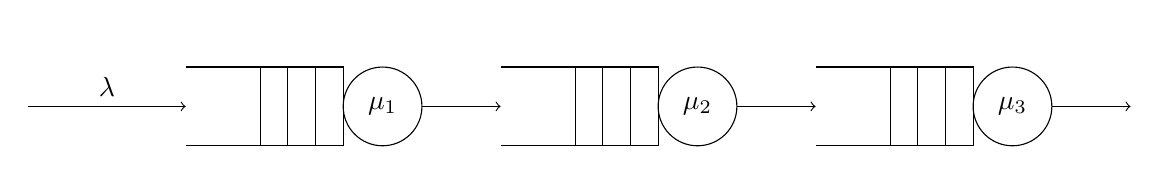
\begin{tikzpicture}[
->-/.style={decoration={markings, mark=at position .5 with {\arrow{stealth}}},
postaction={decorate}},
queuei/.pic={
  \draw%[line width=1pt]
    (0,-0.5) -- ++(2cm,0) -- ++(0,-1cm) -- ++(-2cm,0);
   \foreach \Val in {1,...,3}
     \draw ([xshift=-\Val*10pt]2cm,-0.5) -- ++(0,-1cm);
\draw (2.5,-1) circle [radius=0.5cm] node {#1};}
]
\path 
  (0,1) pic {queuei=$\mu_1$}
  (4,1) pic {queuei=$\mu_2$}
  (8,1) pic {queuei=$\mu_3$};

\draw[->] (-2,0)--(0,0) node[midway, anchor=south] {$\lambda$};
\draw[->] (3,0)--(4,0); 
\draw[->] (7,0)--(8,0); 
\draw[->] (11,0)--(12,0); 
%\draw[->-] (2.5,-0.5)-- ++(0,-1) -- ++(5.,0) -- ++(0, 1.5); 

\end{tikzpicture}

    \caption{Three machines in tandem}
\label{fig:tandemraw}
  \end{figure}

  \begin{solution} 
    The raw processing time is just the sum of the processing times at
    each station. All stations have the same arrival rate, hence
    machine, being the slowest, is the bottleneck. Hence,
 \begin{align*}
      T_0 &= 2 + 3 + 2 = 7\\
   r_b &= \mu_2 = \frac13 \\
      W_0 &= r_b T_0 = \frac73.
    \end{align*}
  \end{solution}
\end{question}


\begin{question}
  A production network consists of 3 single-machine stations in tandem
  with processing times $(2, 3, 2)$ hours.  Suppose we modify this
  network by adding one extra machine to station 2, with processing
  time $t=3$ hours.  What are $W_0$, $r_b$ and $T_0$?
\hint{Is the new machine placed in parallel or in series?}
  \begin{solution}
    Realize that machines at a station are in parallel, not in
    series. Thus, when we add capacity to station 2, we don't add an
    extra processing step to station 2, we increase capacity. 

    Now 
    \begin{equation*}
      r_2 = \frac13 + \frac13 = \frac 23,
    \end{equation*}
    so that station 2 is no longer the bottleneck. Station 1 and
    station 3 are the bottlenecks.
    \begin{align*}
      r_b &= \frac12 \\
      T_0 &= 2 + 3 + 2 = 7\\
      W_0 &= r_b T_0 = \frac72.
    \end{align*}

    Often, students think that the processing rate is the inverse of
    the processing time, i.e., $t=r^{-1}$. This is not the case for
    multi-server stations. Thus, realize that the raw processing time
    at station 2 is still $3$ hours, not $3/2$.
  \end{solution}
\end{question}


\begin{question}
  A production network consists of 3 single-machine stations in tandem
  with processing times $(2, 3, 2)$ hours.  Suppose we modify this
  network by adding one extra machine to station 2 with
  processing time $t=4$ hours.  What are $W_0$, $r_b$ and $T_0$?

\hint{Check your reasoning very carefully here. It is easy to do it wrong.}
\begin{solution}
Now, 
\begin{equation*}
  r_2 = \frac13 + \frac 14 = \frac 7{12} > \frac12,
\end{equation*}
hence, station 1 and 3 are bottlenecks. 


However, $t_2$ cannot be $3$ hours anymore: some jobs will spend 4
hours at station 2 rather than 3 hours. In fact, the computation of
the raw processing time at station 2, $t_2$ say, is a bit tricky. Some
students reason that both machines serve half of the jobs, so that
$T_2=(3+4)/2$ hours.  This, however, is not quite realistic. Like
this, you would load the slow machine all of the time, and the faster
machine would be idle quite a bit of the time. 


  Rather than spreading the jobs evenly over the two machines, we can
  also assume that each machine takes in work in propertion to its
  processing rate.  Then we reason like this. Consider 12 hours. In
  those 12 hours, the slow machine processes 3 jobs with duration 4
  and the fast machine processes 4 jobs with duration 3. Therefore:
  \begin{equation*}
    t_2 = \frac 3 7 4 + \frac 4 7 3 = \frac{24}7.
  \end{equation*}
  Another way to get this is like this. We can `stuff' station 2 with
  jobs. The most jobs that fit in simultaneously is 2, one job per
  machine. Then, with Little's law,
  \begin{equation*}
   t_2 = \frac{W}{r_2} = \frac{2}{7/12} = \frac{24}7,
  \end{equation*}
i.e., the same as the other answer.

Now, finally, 
    \begin{align*}
      r_b &= \frac12 \\
      T_0 &= 2 + \frac{24}7 + 2 = 4 + 3 + \frac37 = 7 \frac37\\
      W_0 &= r_b T_0.
    \end{align*}

    Finally, and the most realistic, is that the fast machine is
    always working, and the slow machine covers the rest.  In that
    case, suppose that the fast machine processes jobs at rate $r_1$
    and the slow at rate $r_2$. Then, since jobs arrive with rate
    $r_a$, the fast machine processes a fraction of $r_1/r_a$ of the
    jobs, and the slow machine processes the left overs, i.e., a
    fraction of $(r_a-r_1)/ra$ of the jobs. The raw processing time then becomes
    \begin{equation*}
      \begin{split}
      t_2 
&= \frac{r_1}{r_a} t_1 + \frac{r_a-r_1}{r_a} t_2 \\
&= \frac{1/3}{1/2} 3 + \frac{1/2-1/3}{1/2} 4 \\
&= 2 + \frac{1/6}{1/2} 4 \\
&= 2 + \frac{4}{3} = 3\frac13,
      \end{split}
    \end{equation*}
and then,
\begin{equation*}
  T_0 = 2 + t_2 + 2 = 7\frac13,
\end{equation*}
and this is a tiny bit less then the previous way of organizing things. 

So, why are the above answers different? One reason is that the
objective is not explicitly stated. It might be that, to minimize time
in a multi-server station, it is optimal to let a fast machine idle
and wait until the next job comes in. If we were to assign this next
job to a slow machine, the time in the system may be longer.  In
general, it might be that schedules that mininime $T_0$ (on average)
are not work-conserving (i.e., such that when jobs are waiting, not
all machines are idle.)
\end{solution}
\end{question}


\begin{question}
Why does the critical WIP change in the different cases above? 
\end{question}
\begin{solution}
  Because $T_0$ increases and/or the bottleneck rate increases. In
  both cases, we need more $W_0$ to fill the network and achieve that
  the throughput can be equal to $r_b$ in the best case.

\end{solution}

\begin{question}
  A production network consists of 3 single-machine stations in tandem
  with processing times $(2, 3, 2)$ hours.  Suppose we modify this
  network by adding one extra machine to station 2 with 
  processing time $t=1$ hour.  What are $W_0$, $r_b$ and $T_0$?
\end{question}
\begin{solution}
  Now the slow machine at station 2 becomes superfluous. The fast
  machine at station 2 can cope with all jobs that arrive from station
  1.
    \begin{align*}
      r_b &= \frac12 \\
      T_0 &= 2 + 1 + 2 = 5\\
      W_0 &= r_b T_0.
    \end{align*}

    Thus, why would you assign part of the jobs to the slow machine at
    station 2? There is no queue, the fast machine can cope with all
    the jobs. Moreover, assigning any job to the slow machines just
    adds to the cycle time.

Taking  $T_2=(1+3)/2=2$ is plainly silly. 
\end{solution}

\begin{question}
  In the previous question, it might seem that one machine at the
  second station is superfluous. Which one, and why? Would you remove
  this superfluous machine in a real production network?
\begin{solution}
  See above. I would not remove the slow machine. In real life there
  is variability: the fast machine might fail for instance. Spare
  capacity is useful. However, if it is very costly to keep the slow
  machine operational, I would scrap it.
\end{solution}
\end{question}


% What would you have
% said if the processing time of the slow machine would have been 5
% hours? Then you simply cannot give half of the jobs to the slow
% machine; it will overflow.

\begin{question}
  A production network consists of 3 single-machine stations in tandem
  with processing times $(2, 3, 2)$ hours.  Suppose we modify this
  network by adding one extra machine to station 2 with processing
  time $t=7$ hours.  What are $W_0$, $r_b$ and $T_0$?
\end{question}
\begin{solution}
  \begin{align*}
  r_2 &= \frac13 + \frac17 = \frac{10}{21} < \frac12\\
\intertext{hence station 2 is still the bottleneck}
T_2 &= \frac{3}{10}7 + \frac{7}{10}3 = \frac{42}{10}=\frac{21}{5}\text{hour}\\
T_0&=2+\frac{21}{5} +2\\
r_b &= \frac{10}{21}\\
W_0 &= r_b T_0.
   \end{align*}

   Note that we add capacity, so that we can process more jobs per
   unit time, but the raw processing time increases!
\end{solution}


\begin{question}
  A production network consists of 3 single-machine stations in tandem
  with processing times $(2, 3, 2)$ hours.  Suppose we modify this
  network such that $2/3$ of the jobs \emph{ leave after the first}
  station, i.e., between station 1 and 2.  What are $W_0$, $r_b$ and
  $T_0$? 
\begin{solution}
  Now there are two loops. One third of the jobs pass all three
  stations. Station 1 can process these job at rate 
  \begin{equation*}
\frac13 r_1 = \frac 13 \frac 12=\frac 16
  \end{equation*}
  per hour. Since this is smaller than $r_2$ and $r_3$, station 1 is
  the bottleneck rate for this loop. Thus, $W_0$ in this loop is
  $r_b T_0 = 1/6\cdot 7 = 7/6$.

  The other loop only contains station 1. The bottleneck rate in this
  loop is 
  \begin{equation*}
r_1\frac23 = \frac12\frac23 = \frac13. 
  \end{equation*}
Thus,
  $W_0 = r_b T_0 = 1/3\cdot 2 = 2/3$ for this loop. 

Hence, the total wip is $7/6 + 2/3 = 11/6$ and
\begin{equation*}
T_0 = \frac13  7 + \frac 23  2=\frac{11}3,
\end{equation*}
since $1/3$ take the long loop with $T=7$ and $2/3$ the short loop
with $T=2$. Thus, $T_0$ is the weighted average raw processing time.

Another way to analyze this situation is like this. Station 1 is the
bottleneck, because its utilization is 1, while
\begin{align*}
  \rho_2 &= \lambda_2 t_2 = \frac12\frac13 3 = \frac 12\\
  \rho_3 &= \lambda_3 t_3 = \frac12\frac13 2 = \frac 13.
\end{align*}
Since station 1 is the bottleneck in this network, $r_b=1/2$. Since
$T_0 = 11/3$, which we obtain as the weigthed average computation
above, we must have that 
\begin{equation*}
W_0 = r_b T_0 = \frac12\frac{11}3 = \frac{11}6, 
\end{equation*}
which agrees with our earlier result.
\end{solution}
\end{question}


\begin{question}
  A production network consists of 3 single-machine stations in tandem
  with processing times $(2, 3, 2)$ hours.  Suppose we modify this
  network such that 4/5 of the jobs \emph{bypass the second} station,
  i.e., 1/5 of the jobs have the routing $[1,2,3]$, but 4/5 have
  routing $[1,3]$.  What are $W_0$, $r_b$ and $T_0$?
\end{question}
\begin{solution}
  Now stations 1 and 3 are bottlenecks with $r_b = 1/2$. For $T_0$ we have
  \begin{equation*}
    T_0 = \frac15 7 + \frac45 4= \frac{23}5.
  \end{equation*}
Thus, 
\begin{equation*}
W_0 = r_b T_0 = \frac 12 \frac{23}5 = \frac{23}{10}.
\end{equation*}
\end{solution}

% \begin{question}
%   Building up on the previous question, which stations would you
%   include anyway in a CONWIP loop, and why?
% \end{question}
% \begin{solution}
%   Now stations 1 and 3 are bottleneck. Thus, both stations need to be
%   part of the conwip loop. For that matter, it is just as easy to also
%   include station 2, and just include all work on the floor in the WIP
%   measurements.
% \end{solution}



\begin{question}
  For the interested: production situations can be pretty
  complicated. Jobs can enter the network at different places, not
  just at station 1 as we considered here. Jobs may also need rework
  at one or more stations. One consequence of these aspects is that
  the slowest machines or stations need not be the bottlenecks. Can
  you find or develop a general algorithm by which we can compute
  $T_0$, $W_0$ and $r_b$ for any network of reasonable size? (I have
  not tried this yet. It might be too difficult. \tbd.) 

  One way to approach this problem is by placing (imaginary) huge
  amounts of work in front of each station and just see how the network drains. 
  \begin{solution}
    As indicated in the problem, I don't have a solution for this
    problem. However, given the elegance of the problem, I am pretty
    sure it has been solved.
  \end{solution}

\end{question}

%%% Local Variables:
%%% mode: latex
%%% TeX-master: "../booktest"
%%% End:
